\documentclass{article}
\pagestyle{empty}
\usepackage{tikz,amsmath}
\usetikzlibrary{arrows,positioning}
\usepackage[margin=1in]{geometry}
\setlength{\parindent}{0in}
\newcommand{\blk}[1]{\rule{.5cm}{0cm}$#1$\rule{.5cm}{0cm}}

\begin{document}
Name\hrulefill Student Number\hrulefill \\
CSCI321, Fall 2017, Pop Quiz \#5

On the following map we are trying to find a path from $A$ to $X$.
Paths and their costs are shown as arcs between nodes.
Heuristic estimates of the distance from a node to $X$ are shown
in the table.  Trace one of the following searches showing the
sorted contents of the open list at each stage.  (Drawing a tree is
optional.)
Each node in the open
list should also be accompanied by its ``value,'' the number that
is used to sort it in the queue.  Break ties alphabetically,
so that if two or more nodes in the open list have the same value, the
one that comes first in the alphabet is removed first.
\begin{itemize}
\item Uniform cost (Dijkstra's) search
\item Best first (greedy) search
\item $A^*$ search.
\end{itemize}

\newcommand{\mynode}[3]{\node[draw,circle,#1 = 1.5cm of #2] (#3) {$#3$}}
\newcommand{\myline}[3]{\draw[->] (#1) -- node[above right]{#2} (#3)}


\begin{tikzpicture}[thick,>=latex]
  \node[draw,circle] (A) {A};
  \mynode{right}{A}{B};
  \mynode{right}{B}{C};
  \mynode{right}{C}{D};
  \mynode{below}{A}{E};
  \mynode{right}{E}{F};
  \mynode{right}{F}{G};
  \mynode{right}{G}{H};
  \mynode{below}{E}{I};
  \mynode{right}{I}{J};
  \mynode{right}{J}{K};
  \mynode{right}{K}{X};
  \myline A9B;
  \myline B8C;
  \myline C2D;
  \myline E6F;
  \myline F1G;
  \myline G8H;
  \myline I7J;
  \myline J8K;
  \myline K3X;
  \myline A5E;
  \myline B2F;
  \myline C3G;
  \myline D9H;
  \myline E3I;
  \myline F4J;
  \myline G1K;
  \myline H5X;
\end{tikzpicture}
\hfill
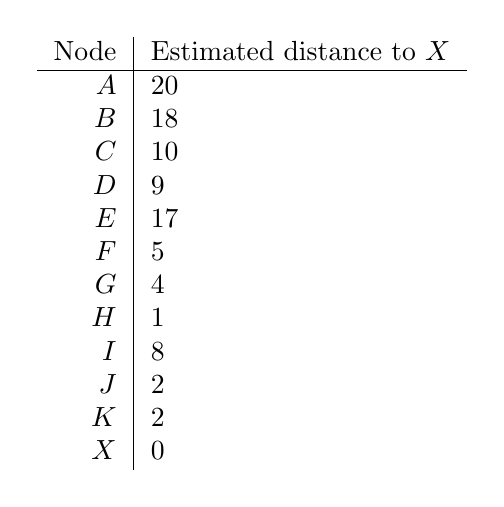
\begin{tikzpicture}
  \node {
\begin{tabular}{r|l}
  Node & Estimated distance to $X$ \\\hline
  $A$ & 20 \\
  $B$ & 18 \\
  $C$ & 10 \\
  $D$ & 9 \\
  $E$ & 17 \\
  $F$ & 5 \\
  $G$ & 4 \\
  $H$ & 1 \\
  $I$ & 8 \\
  $J$ & 2 \\
  $K$ & 2 \\
  $X$ & 0
  \end{tabular}
  };
\end{tikzpicture}




\end{document}
